\begin{answer}{coin100flipsgamble}
This can be solved by using the Central Limit Theorem, or the normal approximation the binomial distribution.
\index{Tricks!Central Limit Theorem}
We have
\begin{align*}
  Y \sim \text{Binomial}(p=0.5, n=100)
\end{align*}
and for large $n$ we can approximate the binomial distribution through the normal distribution, \begin{align*}
  Y &\stackrel{\sim}{\text{\tiny approx}}  \text{Normal}(np, np(1-p))
  \text{.}
\end{align*}
The values of $n$ and $p$ in the problem give
\begin{align*}
  np      &= 100\left(\nicefrac{1}{2}\right)    = 50\\
  np(1-p) &= 100\left(\nicefrac{1}{2}\right)^2  = 25
  \text{,}
\end{align*}
resulting in
\begin{align*}
  Y & \sim
  \text{Normal}\left( 50, (5)^2 \right)
  \text{.}
\end{align*}

In order to evaluate whether the gamble is worthwhile we have to calculate its expected return:
\begin{align*}
  \E(\text{Gamble}) &= -1 + (10)P(\text{Win})  + (0)P(\text{Lose}) \\
                    &= -1 + (10)P(Y>60)
                    \text{.}
\end{align*}
Since we are in an interview, we need to evaluate $P(Y>60)$ without a calculator.
\index{Tricks!Normal probabilities in your head}
With the normal distribution, approximately 95\% of the data lies within two standard deviations of the mean.
For our problem, two standard deviations from the mean is conveniently located at 60, as the following graph indicates.
\begin{center}
  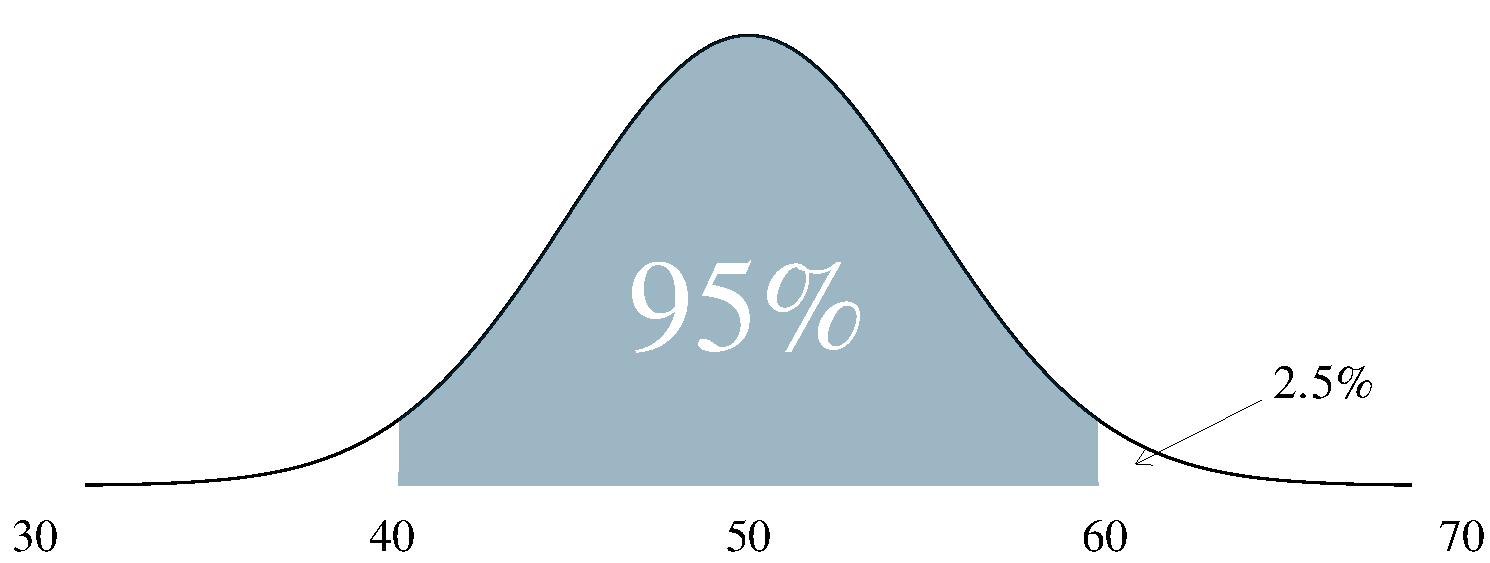
\includegraphics[width=0.8\textwidth]{./plots/prettynorm/prettynorm.pdf}
\end{center}
The probability of interest is $P(Y>60 = 0.025)$ and thus the expected value of our gamble is
\[
  \E(\text{Gamble}) = -1 + (10)(0.025) = 1 - 0.25 = -0.75
  \text{.}
\]
On average we lose 75 pence for playing the game so it is not worthwhile.
The fair price, denoted $\pounds_{\text{fair}}$, occurs where the gamble breaks even:
\begin{align*}
  \E(\text{Gamble})     &=  0    \\
  \pounds_{\text{fair}} - 0.25 &=  0    \\
  \pounds_{\text{fair}}        &=  0.25
\end{align*}
and this is the highest price at which a
rational and risk-neutral person should start agreeing to partake in it.
The assumptions of rationality and risk neutrality are very important.
If a billionaire gets immeasurable physical pleasure from engaging in risky gambles (meaning they aren't risk neutral), the rational course of action for them is probably to spend all of their excess money on unfair gambles.
Conversely, risk-neutral people might not always act rational.

\end{answer}
